\documentclass[10pt]{article}
\usepackage{array}
\usepackage{comment}
\usepackage{fullpage}
\usepackage{pbox}
\usepackage{amssymb}
\usepackage{latexsym}
\usepackage{bm}
\usepackage{amsfonts}
\usepackage{amsmath}
\usepackage{graphicx}
\usepackage{listings}

\usepackage[sectionbib,round]{natbib}


\begin{document}
\section{Alphabet and its uses}

\begin{tabular}{p{3cm} p{13cm}}
Terminologies: & terms, coefficients, arguments, degree, factor, dependent variable, independent variable, free constants, fixed constants, variables, vector, function, counter, bounding element, locus, enumeration, frustum (frustum of right circular cone), heuristic (discovering), if...then...hence, permutations, combinations\\\\
\end{tabular}
\\\\
\begin{tabular}{p{3cm} p{13cm}}
Notations: & $\underbrace{\text{a b c}}_{\text{free constants}}$ \hspace{6pt}
$\underbrace{\text{d e}}_{\text{reserved constants}}$ \hspace{6pt}
$\underbrace{\text{f g h}}_{\text{functions}}$ \hspace{6pt}
$\underbrace{\text{i j k}}_{\text{imaginary vector}}$ \hspace{6pt}
$\underbrace{\text{l m n}}_{\text{reserved for counter}}$ \hspace{6pt}
$\underbrace{\text{o p q r s t}}_{\text{physical constant}}$  \hspace{6pt}
$\underbrace{\text{u v w}}_{\text{auxilliary functions}}$ \hspace{6pt}
$\underbrace{\text{w y z}}_{\text{axis of coordinates}}$\\\\
\end{tabular}
\\\\


\begin{tabular}{p{3cm} p{1cm} p{1cm} p{1cm} p{1cm} p{1cm} p{1cm} p{1cm} p{1cm}}

Space: & point & line & plane & space & \dots & segment & triangle & tetrahedron \\
       & $R^0$ & $R^1$ & $R^2$ & $R^3$ & \dots & lines & polygon & polyhedron \\
\end{tabular}

\subsubsection*{Greek letters and numerals}

\begin{tabular}{p{1.5cm} p{1.5cm} p{1.5cm} p{1.5cm} p{2cm} p{1.8cm} p{1.8cm}  p{1.5cm}}
%\multicolumn{9}{c}{join} \\
\bf{Alphabet} &  &  &  &  & \# & \bf{Greek} & \bf{Latin} \\

$\alpha A$ & alpha & $\backslash$alpha & A &  & 1/2 & hemi- & uni- \\
$\beta B$ & beta & $\backslash$beta   & B &  & 1 & hen-  \\
$\gamma \Gamma$ & gamma & $\backslash$gamma & $\backslash$Gamma &  & 2 & di-,dy-,duo- & du- \\
$\delta \Delta$ & delta & $\backslash$delta & $\backslash$Delta &  & 3 & tri- &tri-\\
$\epsilon \varepsilon E$ & epsilon & $\backslash$epsilon & $\backslash$varepsilon & E   & 4 & tetra- & quadri- \\
$\zeta Z$ & zeta & $\backslash$zeta & Z &   & 5 & penta- & quinque-\\
$\eta H$ & eta & $\backslash$eta & H &   & 6 & hexa- &sexa-\\
$\theta \vartheta \Theta$ & theta & $\backslash$theta & $\backslash$vartheta & $\backslash$Theta   & 7 & hepta- & septem-, septi\\
$\iota I$ & iota & $\backslash$iota & I &   & 8 & octa-,octo- & octo-\\
$\kappa K$ & kappa & $\backslash$kappa & K &   & 9 & ennea- & novem- \\
$\lambda \Lambda $ & lambda & $\backslash$lambda & $\backslash$Lambda &   & 10 & deca- & dec-\\
$\mu M $ & mu & $\backslash$mu & M &   & 100 & hecato- & centi- \\
$\nu N $ & nu & $\backslash$nu & N &   &  1000  & chilia- & milli-\\
$\xi \Xi $ & xi & $\backslash$xi & $\backslash$Xi &   & Unspecified & poly- & multi-\\
$o O $ & omikron & $o$ & $O$ &   &   \\
$\pi \Pi $ & pi & $\backslash$pi & $\backslash$Pi &   &   &\\
$\rho \varrho P $ & rho & $\backslash$rho & $\backslash$varrho & P   &   &\\
$\sigma \Sigma $ & sigma & $\backslash$sigma & $\backslash$Sigma &   &   &\\
$\tau T $ & tau & $\backslash$tau & T & & \\
$\upsilon \Upsilon $ & upsilon & $\backslash$upsilon & $\backslash$Upsilon & &\\
$\phi \varphi \Phi $ & phi & $\backslash$phi & $\backslash$varphi & $\backslash$Phi &\\
$\chi X$ & chi & $\backslash$chi & X & &\\
$\psi \Psi $ & psi & $\backslash$psi & $\backslash$Psi & &\\
$\omega \Omega $ & omega & $\backslash$omega & $\backslash$Omega & &\\\\
\end{tabular}
\\\\
\subsubsection*{Number sets}
\begin{tabular}{p{1.5cm} p{3.4cm} p{2cm} p{2cm} p{2cm} p{2cm}}
$\mathbb{P}$ & prime numbers & $\backslash$mathbb$\lbrace \text{P} \rbrace$ & & &\\
$\mathbb{N}$ & natural numbers & $\backslash$mathbb$\lbrace \text{N} \rbrace$ & & &\\
$\mathbb{Z}$ & integers & $\backslash$mathbb$\lbrace \text{Z} \rbrace$ & & &\\
$\mathbb{I}$ & irrational numbers & $\backslash$mathbb$\lbrace \text{I} \rbrace$ & & &\\
$\mathbb{Q}$ & rational numbers & $\backslash$mathbb$\lbrace \text{Q} \rbrace$ & & &\\
$\mathbb{R}$ & real numbers & $\backslash$mathbb$\lbrace \text{R} \rbrace$ & & &\\
$\mathbb{C}$ & complex numbers & $\backslash$mathbb$\lbrace \text{C} \rbrace$ & & &\\
\end{tabular}
%\begin{tabular}{c c c c c c c c c}
%\multicolumn{9}{c}{join} \\
%\multicolumn{3}{c}{First Long Text} &
%\multicolumn{3}{c}{Second Long Text} &
%\multicolumn{3}{c}{a} \\
%\hspace{50pt}  & \hspace{50pt} & \hspace{50pt} &  &  &  &  &  &  \\
%\end{tabular}
%\textbf{1.4 Definitions: All rational numbers is denoted as $\mathbb{Q}$}
\\\\\\
\begin{tabular}{p{3cm} p{13cm}}
n-space \hspace{2cm} and n-dimension &
There is an important distinction between the coordinate n-space R$^n$ and a general finite-dimensional vector space $V$. While R$^n$ has a standard basis $\{ e_1, e_2, ..., e_n \}$, a vector space $V$ typically does not come equipped with such a basis and many different bases exist (although they all consist of the same number of elements equal to the dimension of $V$). \cite{wiki_LA}
\begin{verbatim}
(Wikipedia contributors. Linear algebra. Wikipedia, The Free Encyclopedia. 
May 6, 2016, 15:18 UTC. Available at: https://en.wikipedia.org/w/index.php?
title=Linear_algebra&oldid=718937296. Accessed May 18, 2016.)
\end{verbatim}
\end{tabular}
\\\\
\begin{tabular}{p{3cm} p{13cm}}
Notation \hspace{2cm} & Tips on how to name your constants, variables, data and unknowns: \\
 Remarks by Polya & $\cdot$ Consecutive letters should be used as symbols when symbols represent same category. For examples a,b,c for constants and x,y,z for variables. \\
& 
$\cdot$ Use first letter of its name for the symbol. For examples r for radius, l for length, w for width. Notice that this method is more specific than the first method mentioned.\\ 
& $\cdot$ Use same letter from different alphabets when these are related mathematically, intuitively, or even plausibly. For examples,\\
& \hspace{1cm} Roman capitals such as A, B, C, $\ldots$, for points.\\
& \hspace{1cm} small Roman letters such as a, b, c, $\ldots$, for lines.\\
 & \hspace{1cm} Greek letters such as $\alpha, \beta, \gamma$, $\ldots$, for angles.\\
 & \hspace{1cm} You want A, a, $\alpha$ to be connected some ways. For example A and $\alpha$ to represent the same vertex and a to be adjacent edge from A.\\
 & \begin{center} 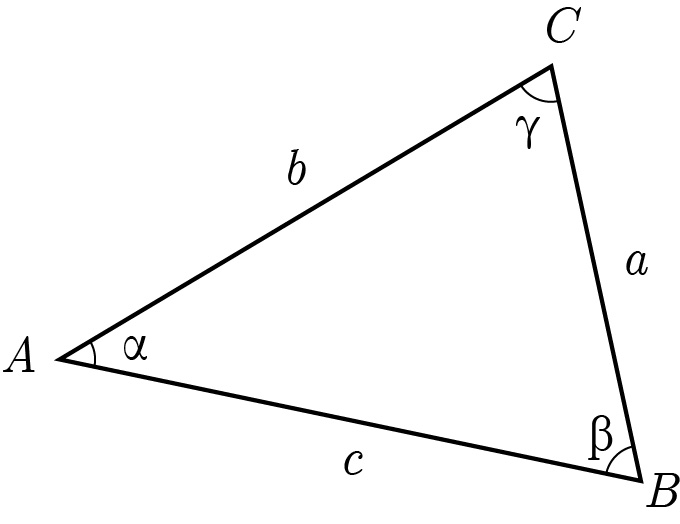
\includegraphics[width=1in]{Capture5.jpg} \end{center}\\
 & Note: These remarks are very much related to how to name classes and functions in programming language. Apply useful tips interchangeably.\\
   
\end{tabular}
\end{document}
